\documentclass{article}
%\usepackage{babel}
\usepackage{tikz}
\usepackage{comment}
\usepackage{multicol}
\usepackage{amsmath}
\usepackage{amssymb,amsfonts,amsthm}
\usepackage{amsthm,textcomp}
%\usepackage[top=2cm, bottom=2cm, left=2in, right=1in]{geometry}

%\textheight = 692pt

\newcommand{\setup}{
    \coordinate (z0) at (0,0);
    \coordinate (z1) at (4,0);
    \coordinate (z2) at (2,1);
    \coordinate (z3) at (6,1);

    \coordinate (z4) at (0,4);
    \coordinate (z5) at (4,4);
    \coordinate (z6) at (2,5);
    \coordinate (z7) at (6,5);
}

\newcommand{\mycube}[1]{
    \tikzstyle{every node}=[font=\Large]

    \draw[line width=#1 pt] (z0) rectangle (z5); % face rectangle
    \draw[line width=#1 pt,dashed] (z2) -- (z3);
    \draw[line width=#1 pt,dashed] (z2) -- (z6);
    \draw[line width=#1 pt] (z3) -- (z7);
    \draw[line width=#1 pt] (z6) -- (z7);

    \draw[line width=#1 pt,dashed] (z0) -- (z2);
    \draw[line width=#1 pt] (z1) -- (z3);
    \draw[line width=#1 pt] (z4) -- (z6);
    \draw[line width=#1 pt] (z5) -- (z7);
    
    \node[below left =2pt] at (z0) {$z_0$};
    \node[below left =4pt] at (z1) {$z_1$};
%    \node[above right=3pt] at (z2) {$z_2$};
    \node[below      =3pt] at (z2) {$z_2$};
    \node[above right=2pt] at (z3) {$z_3$};

    \node[above left =2pt] at (z4) {$z_4$};
    \node[above left =2pt] at (z5) {$z_5$};
    \node[above right=3pt] at (z6) {$z_6$};
    \node[above right=2pt] at (z7) {$z_7$};
} 

\newcommand{\fillDots}[4]{
  \fill (#1) circle (2.5pt);
  \fill (#2) circle (2.5pt);
  \fill (#3) circle (2.5pt);
  \fill (#4) circle (2.5pt);
}

\begin{document}

  \section{Geometry}
  
  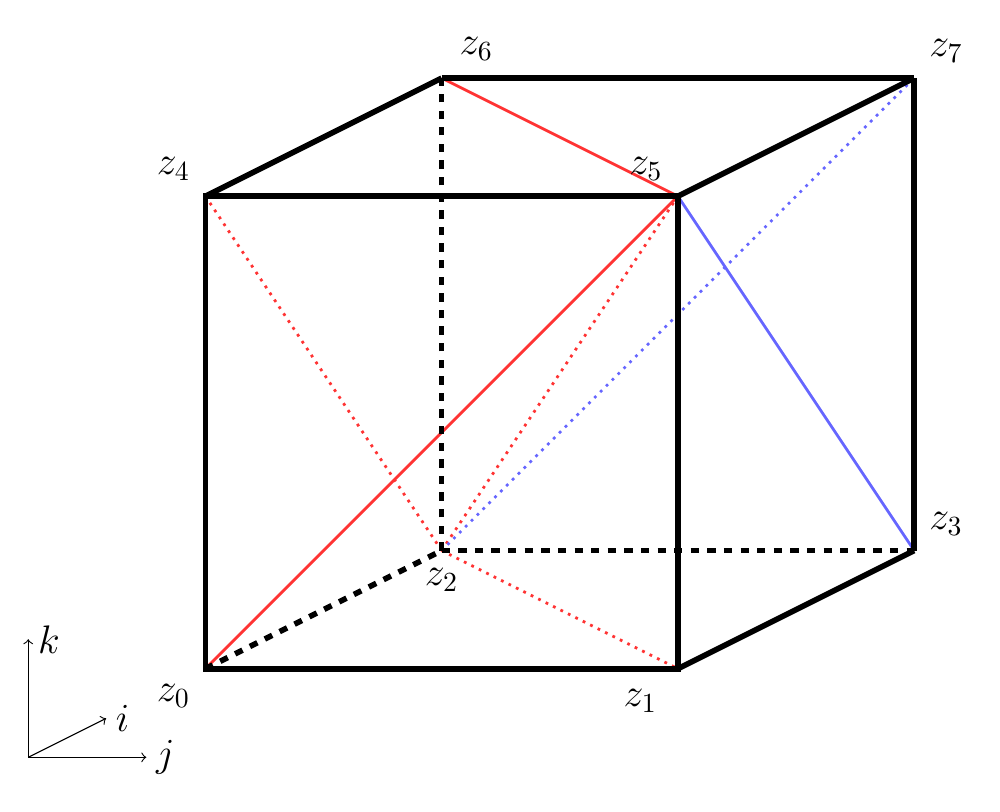
\begin{tikzpicture}[scale=1.5]
    \setup;

    \draw[line width=1pt,dotted,red!80] (z2) -- (z5);
    
    \draw[line width=1pt,red!80]  (z5) -- (z0);
    \draw[line width=1pt,blue!60] (z5) -- (z3);
    \draw[line width=1pt,red!80]  (z5) -- (z6);

    \draw[line width=1pt,dotted,red!80]  (z2) -- (z1);
    \draw[line width=1pt,dotted,red!80]  (z2) -- (z4);
    \draw[line width=1pt,dotted,blue!60] (z2) -- (z7);

    \mycube{2};
    
    \coordinate (o) at (-1.5,-0.75);
    \draw[->] (o) -- ++(1,0)        node[right] {$j$};
    \draw[->] (o) -- ++(0.66, 0.33) node[right] {$i$};
    \draw[->] (o) -- ++(0,1)        node[right] {$k$};
  \end{tikzpicture}

  \section{Element stiffness matrix}
  
  { \LARGE
  $$
  \bordermatrix{ 
                & z_0 & z_1 & z_2 & z_3 & z_4 & z_5 & z_6 & z_7     \cr
            z_0 &  4  & -1  & -2  &     & -1  &     &     &         \cr
            z_1 & -1  &  4  &     & -1  &     & -2  &     &         \cr
            z_2 & -2  &     &  6  & -2  &     &     & -2  &         \cr
            z_3 &     & -1  & -2  &  4  &     &     &     & -1      \cr
            z_4 & -1  &     &     &     &  4  & -2  & -1  &         \cr
            z_5 &     & -2  &     &     & -2  &  6  &     & -2      \cr
            z_6 &     &     & -2  &     & -1  &     &  4  & -1      \cr
            z_7 &     &     &     & -1  &     & -2  & -1  &  4 
  }
  $$
  }
  
  \newpage
  
  \begin{figure}[hb]
    \begin{minipage}[c]{7cm}
      \hspace{-3cm}
      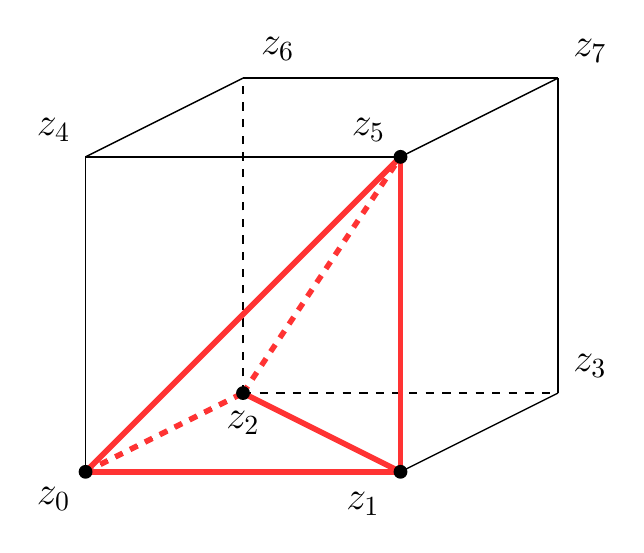
\begin{tikzpicture}[scale=1]
          \setup;
          \mycube{0.5};

          \draw[line width=2pt,dashed,red!80] (z2) -- (z5);
          \draw[line width=2pt,red!80] (z2) -- (z1);
          \draw[line width=2pt,red!80] (z5) -- (z0);
          \draw[line width=2pt,dashed,red!80] (z0) -- (z2);
          \draw[line width=2pt,red!80] (z0) -- (z1);
          \draw[line width=2pt,red!80] (z5) -- (z1);

          
          \fillDots{z0}{z1}{z2}{z5};
        \end{tikzpicture}
    \end{minipage}
    \begin{minipage}[c]{7cm}
    { \Large
    $(z_0 \ z_1 \ z_2 \ z_5 )$
    
    $$
      \bordermatrix{ 
                    & z_0 & z_1 & z_2 & z_5     \cr
                z_0 &  2  & -1  & -1  &         \cr
                z_1 & -1  &  2  &     & -1      \cr
                z_2 & -1  &     &  1  &         \cr
                z_5 &     & -1  &     &  1
      }
    $$
    }
    \end{minipage}
%  \end{figure}

%  \begin{figure}[hb]
    \begin{minipage}[c]{7cm}
      \hspace{-3cm}
      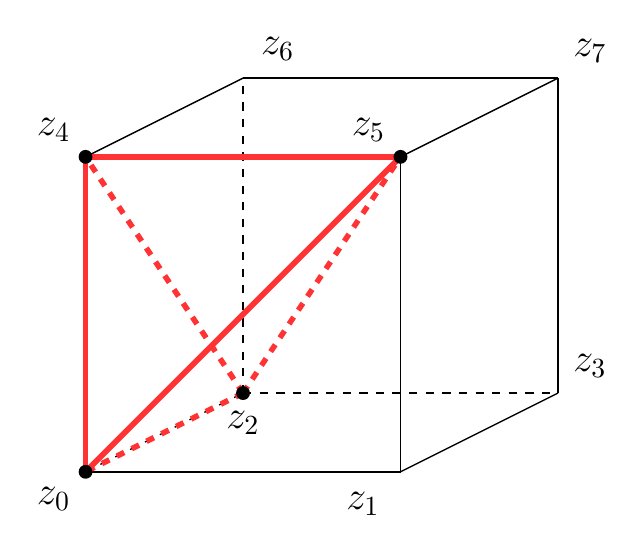
\begin{tikzpicture}[scale=1]
          \setup;
          \mycube{0.5};

          \draw[line width=2pt,dashed,red!80] (z2) -- (z0);
          \draw[line width=2pt,dashed,red!80] (z2) -- (z5);
          \draw[line width=2pt,dashed,red!80] (z2) -- (z4);
          \draw[line width=2pt,red!80] (z0) -- (z4);
          \draw[line width=2pt,red!80] (z0) -- (z5);
          \draw[line width=2pt,red!80] (z4) -- (z5);

          
          \fillDots{z0}{z2}{z4}{z5};
        \end{tikzpicture}
    \end{minipage}
    \begin{minipage}[c]{7cm}
    { \Large
    $(z_0 \ z_2 \ z_4 \ z_5 )$
    
    $$
      \bordermatrix{ 
                    & z_0 & z_2 & z_4 & z_5     \cr
                z_0 &  2  & -1  & -1  &         \cr
                z_2 & -1  &  1  &     &         \cr
                z_4 & -1  &     &  2  & -1      \cr
                z_5 &     &     & -1  &  1
      }
    $$
    }
    \end{minipage}
%  \end{figure}

%  \begin{figure}[hb]
    \begin{minipage}[c]{7cm}
      \hspace{-3cm}
      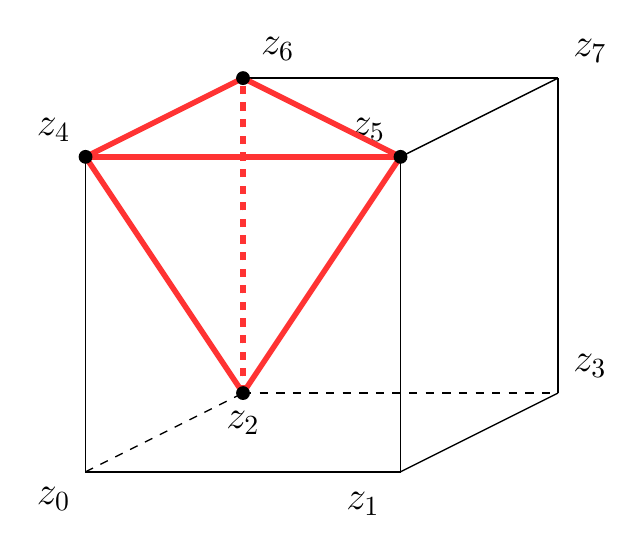
\begin{tikzpicture}[scale=1]
          \setup;
          \mycube{0.5};

          \draw[line width=2pt,dashed,red!80] (z2) -- (z6);
          \draw[line width=2pt,red!80] (z2) -- (z5);
          \draw[line width=2pt,red!80] (z2) -- (z4);
          \draw[line width=2pt,red!80] (z4) -- (z5);
          \draw[line width=2pt,red!80] (z4) -- (z6);
          \draw[line width=2pt,red!80] (z5) -- (z6);

          
          \fillDots{z2}{z4}{z5}{z6};
        \end{tikzpicture}
    \end{minipage}
    \begin{minipage}[c]{7cm}
    { \Large
    $(z_2 \ z_4 \ z_5 \ z_6 )$
    
    $$
      \bordermatrix{ 
                    & z_2 & z_4 & z_5 & z_6     \cr
                z_2 &  1  &     &     & -1      \cr
                z_4 &     &  2  & -1  & -1      \cr
                z_5 &     & -1  &  1  &         \cr
                z_6 & -1  & -1  &     &  2
      }
    $$
    }
    \end{minipage}
  \end{figure}

  \begin{figure}[hb]
    \begin{minipage}[c]{7cm}
      \hspace{-3cm}
      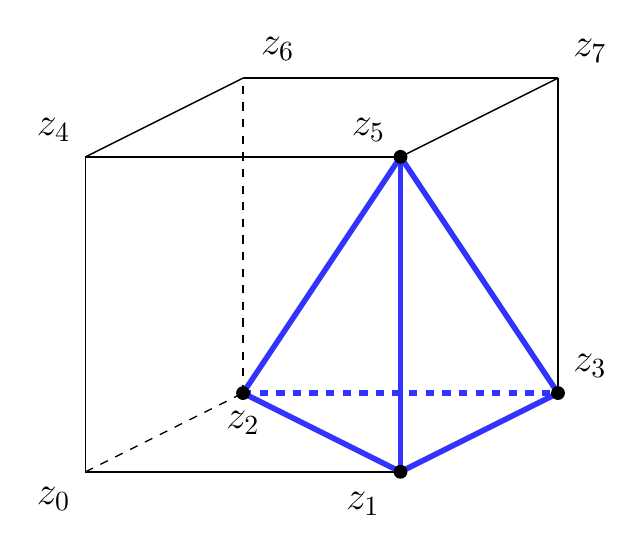
\begin{tikzpicture}[scale=1]
          \setup;
          \mycube{0.5};

          \draw[line width=2pt,dashed,blue!80] (z2) -- (z3);
          \draw[line width=2pt,blue!80] (z1) -- (z2);
          \draw[line width=2pt,blue!80] (z1) -- (z3);
          \draw[line width=2pt,blue!80] (z1) -- (z5);
          \draw[line width=2pt,blue!80] (z5) -- (z3);
          \draw[line width=2pt,blue!80] (z5) -- (z2);
          
          \fillDots{z1}{z2}{z3}{z5};
        \end{tikzpicture}
    \end{minipage}
    \begin{minipage}[c]{7cm}
    { \Large
    $(z_1 \ z_2 \ z_3 \ z_5 )$
    
    $$
      \bordermatrix{ 
                    & z_1 & z_2 & z_3 & z_5     \cr
                z_1 &  2  &     & -1  & -1      \cr
                z_2 &     &  1  & -1  &         \cr
                z_3 & -1  & -1  &  2  &         \cr
                z_5 & -1  &     &     &  1
      }
    $$
    }
    \end{minipage}
%  \end{figure}

%  \begin{figure}[hb]
    \begin{minipage}[c]{7cm}
      \hspace{-3cm}
      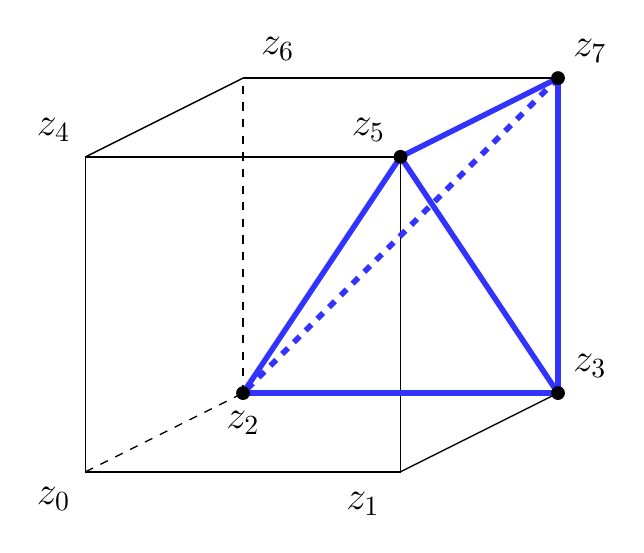
\begin{tikzpicture}[scale=1]
          \setup;
          \mycube{0.5};

          \draw[line width=2pt,dashed,blue!80] (z7) -- (z2);
          \draw[line width=2pt,blue!80] (z2) -- (z3);
          \draw[line width=2pt,blue!80] (z5) -- (z3);
          \draw[line width=2pt,blue!80] (z5) -- (z2);
          \draw[line width=2pt,blue!80] (z5) -- (z7);
          \draw[line width=2pt,blue!80] (z7) -- (z3);

          
          \fillDots{z2}{z3}{z5}{z7};
        \end{tikzpicture}
    \end{minipage}
    \begin{minipage}[c]{7cm}
    { \Large
    $(z_2 \ z_3 \ z_5 \ z_7 )$
    
    $$
      \bordermatrix{ 
                    & z_2 & z_3 & z_5 & z_7     \cr
                z_2 &  1  & -1  &     &         \cr
                z_3 & -1  &  2  &     & -1      \cr
                z_5 &     &     &  1  & -1      \cr
                z_7 &     & -1  & -1  &  2
      }
    $$
    }
    \end{minipage}
%  \end{figure}

%  \begin{figure}[hb]
    \begin{minipage}[c]{7cm}
      \hspace{-3cm}
      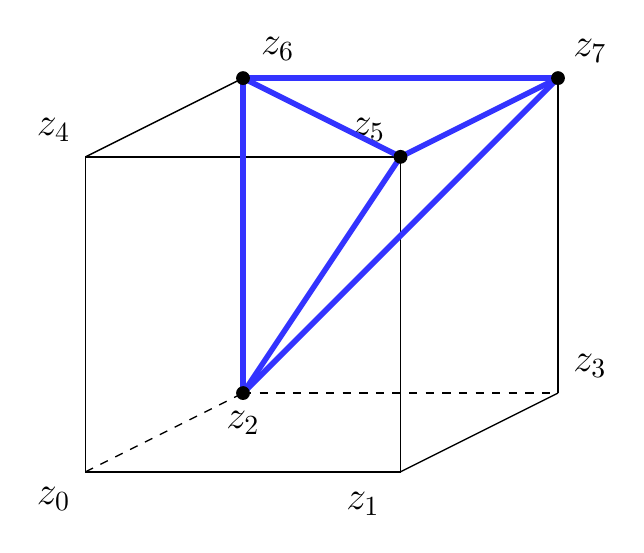
\begin{tikzpicture}[scale=1]
          \setup;
          \mycube{0.5};

          \draw[line width=2pt,blue!80] (z2) -- (z6);
          \draw[line width=2pt,blue!80] (z2) -- (z7);
          \draw[line width=2pt,blue!80] (z5) -- (z2);
          \draw[line width=2pt,blue!80] (z5) -- (z6);
          \draw[line width=2pt,blue!80] (z5) -- (z7);
          \draw[line width=2pt,blue!80] (z6) -- (z7);

          
          \fillDots{z2}{z5}{z6}{z7};
        \end{tikzpicture}
    \end{minipage}
    \begin{minipage}[c]{7cm}
    { \Large
    $(z_2 \ z_5 \ z_6 \ z_7 )$
    
    $$
      \bordermatrix{ 
                    & z_2 & z_5 & z_6 & z_7     \cr
                z_2 &  1  &     & -1  &         \cr
                z_5 &     &  1  &     & -1      \cr
                z_6 & -1  &     &  2  & -1      \cr
                z_7 &     & -1  & -1  &  2
      }
    $$
    }
    \end{minipage}
  \end{figure}

\end{document}
